\documentclass[twoside]{article}

\usepackage{ustj}

\addbibresource{mss.bib}

\newcommand{\authorname}{Phillip C. Monk}
\newcommand{\authorpatp}{\patp{wicdev-wisryt}}
\newcommand{\affiliation}{Tlon Corporation}

%  Make first page footer:
\fancypagestyle{firststyle}{%
\fancyhf{}% Clear header/footer
\fancyhead{}
\fancyfoot[L]{{\footnotesize
              %% We toggle between these:
              Manuscript submitted for review.\\
              % {\it Urbit Systems Technical Journal} I:2 (2024):  1–6. \\
              ~ \\
              Address author correspondence to \authorpatp.
              }}
}
%  Arrange subsequent pages:
\fancyhf{}
\fancyhead[LE]{{\urbitfont Urbit Systems Technical Journal}}
\fancyhead[RO]{The {\sc pki} Idea Maze}
\fancyfoot[LE,RO]{\thepage}

%%MANUSCRIPT
\title{Designing a Permanent Personal Identity: \\ The Public Key Infrastructure Idea Maze}
\author{\authorname~\authorpatp \\ \affiliation}
\date{}

\begin{document}

\maketitle
\thispagestyle{firststyle}

\begin{abstract}
\sloppy
Public key infrastructures solve a coordination problem for communicators on a network. Urbit's {\sc pki} (Azimuth) is designed to provide globally consistent, permanent, and completely self-owned identities. This post explores the design choices that led to Urbit's {\sc pki}, including the trade-offs between impermanence and self-attestation, global consistency, and scalability. Urbit's {\sc pki} includes three types of names epitomizing the poles of the tradeoff trilemma.
\end{abstract}

% We will adjust page numbering in final editing.
\pagenumbering{arabic}
\setcounter{page}{1}

% \tableofcontents

A public key infrastructure ({\sc pki}) is a system for binding a set of keys to a name. Sometimes a small amount of metadata is included. Existing {\sc pki}s include {\sc pgp}-style
\href{https://en.wikipedia.org/wiki/Web_of_trust}{``web of trust''},
\href{https://en.wikipedia.org/wiki/Certificate_authority}{{\sc ssl}
certificates},
\href{https://www.zerotier.com/lf-announcement/}{ZeroTier},
\href{https://keybase.io/}{Keybase},
\href{https://openid.net/what-is-openid/}{OpenID},
\href{https://developer.mozilla.org/en-US/docs/Archive/Mozilla/Persona}{Mozilla
Persona}, and \href{https://developers.google.com/identity}{Login with
Google}. These take unique approaches to the problem and have achieved
some degree of success, but none provide globally consistent, permanent,
and completely self-owned identities. In this article, we will describe Urbit's approach to achieving these properties in its {\sc pki}.

Urbit's {\sc pki} is named ``Azimuth'' (or occasionally ``Urbit ID'').  Azimuth is Urbit's identity layer, built as a suite of smart contracts on the Ethereum blockchain and several apps run locally on your ``ship''. (In Urbit, a ``name'' is often called a ``ship'' or an ``address''
because we use the metadata in the {\sc pki} to make names routable.) The total
data is two 256-bit asymmetric keys, a cryptographic suite number (to
allow changing crypto algorithms), the revision number of the key, and
the name of a ship that will route for it. This sums to less than 128
bytes of data.

Each {\sc pki} trades off various properties. We chose a tripartite system so
that appropriate choices can be made for different use cases. Here, we
explore the various properties we chose by following a series of binary
choices—the idea maze.

One way to classify {\sc pki}s is by permanence: either you can change your keys or not. If
you cannot, then your name is impermanent, for no one can keep a set of
keys secure forever. Even if your opsec never fails, eventually your
crypto algorithms may be compromised.

However, if you sacrifice the ability to change your keys, you can achieve
a very nice property: self-attesting keys. If your name is a hash of
your public key information, then no other source of information is
required to verify you are who you say you are. This is a useful
property since it requires no coordination at all. Many things are
impermanent, especially during development. It also provides a way to
try out the network without obtaining a permanent address.

This is our first stop in the idea maze. We call this sort of name a
``comet''. A comet's name is the 128-bit hash of its public keys.\footnote{We currently limit comets to ``sponsors'', particular stars which are whitelisted to create them.  This is a matter of policy and not inherent to the {\sc pki} design.}

However, Urbit is yours and it's forever. You shouldn't have to change
your name every time you change your keys. So, we go back and take the
other choice: you must be able to change your keys.

To change keys, you must sign a message with the old keys revoking them
and supplying the new
ones\footnote{Or the equivalent with a hierarchical key structure. In practice, you
want to have a master key which signs a junior key for everyday use.
You use the master key to rotate the junior
key.}. The question is what
happens if the old keys also sign a second set of new keys. This could
happen if an attacker obtained your old keys after the fact. This is
important because one of the reasons to be able to change your keys is
to invalidate the old ones so that they have no power.

We have two options again: the {\sc pki} may be globally consistent or not. To
be globally consistent means that if you believe a name is bound to a
set of keys, then nobody on the network will disagree.

If you don't require global consistency, you may sign this message and
send it to all your neighbors, and they pass it on, and hopefully it
gets to most of the network quickly. However, if one of those ships
receives two contradictory versions of this message, the only thing it
can do is trust the first one it heard, which may be different than what
someone else heard. Thus, this is pairwise consistent but globally
inconsistent. This is essentially how the pre-blockchain Ames network
worked, though key changes were not actually implemented. Because global
consistency is a valuable property, we looked at other options.

For a globally consistent {\sc pki} that allows you to revoke keys, you need
to be able to distinguish between two cryptographically valid messages
to determine which was signed first. The dual problem could be solved
easily --- you can prove a message is signed after another by including
the signature of the first in the second. This is equivalent to reading
out a newspaper headline to prove a message was recorded after a given
day.

However, the problem of proving one message was sent before any later
ones inverts the problem. You can solve this with newspapers by placing
the message in the text of the newspaper. However, while reading a
newspaper requires no central party, writing one does. For a long time,
this sort of message was always handled by a central party. {\sc ssl}
revocations are managed by a few central parties. When you buy property,
it's not sufficient to have the previous owner sign the title --- this
must be entered into a central land registry. Otherwise, the owner may
sell their property to multiple people and there would be no way to
determine who is the new owner. With the land registry, all you need to
do is ask the registry which sale happened first, and that's the one
that counts.

However, Urbit is yours and it's forever. Trusting central registries
jeopardizes both. The keen reader will notice that the problem of
determining which key rotation happened first is exactly the
double-spend problem that Satoshi solved with his proof of work
algorithm for Bitcoin. His first block famously includes a newspaper
headline to prove he didn't mine the block before that date. In a
beautiful duality, his own algorithm proves that he didn't mine it after
that date.\footnote{More strictly: it proves that he didn't mine it after the other blocks
currently on the Bitcoin blockchain. It only gives an ordering within
the chain, not a literal
timestamp.  But cf. \citet{Gigi2019} and particularly \citet{Gigi2021} on Bitcoin ordering as time.}

Some argue that blockchain is only good for money. This is myopic and is
generally based on the experience that its most valuable application so
far has been money. However, blockchain is a cryptographic primitive to
do what was previously impossible: prove that one message was signed
before another without a central party. Blockchain was discovered by
someone trying to create digital money, and he needed that primitive,
but that doesn't mean that's all it's good for.

Thus, we store our {\sc pki} data on a blockchain for our second kind of name:
planets. A planet is a 32-bit address which has key information stored
on the blockchain.\footnote{In addition to planets, there are stars and galaxies. From a {\sc pki}
perspective they're treated exactly like planets, but on the network
they provide infra\-structure services like
routing.} The
owner of a planet may broadcast new {\sc pki} data by adding it to the
blockchain. Any later messages by the old keys will be rejected, and
everyone on the network will listen to the blockchain for key data.
Thus, we have global consistency, permanence, and self sovereignty. We
know of no other solution that can provide these properties.

However, while small individually, the aggregate {\sc pki} data for all nodes
on the network may become very large. This is not an issue for comets
because nobody needs to store comet keys except for those which they're
talking with, and even those can be garbage-collected and re-requested
and verified. For planets, there is a canonical set of keys, and
somebody must store that. There are about 232, or 4 billion planets. If
the {\sc pki} data is about 100 bytes for each planet, this is about 400 GB of
data. This may be more than most users wish to store, but it's small
enough that it would be very cheap for someone to host this data for
many users.\footnote{In practice, this will likely be an included service by your
sponsoring star. It should never rise above the capital cost of a
400GB hard drive.}

\sloppy
This information is currently stored directly on the Ether\-eum blockchain, but as is well understood in blockchain circles this
approach will not scale beyond a certain point. Many chains are pursuing
designs that allow the users of the smart contracts to locally store the
data associated with the contracts they care about and only commit
hashes to the chain. We expect there to be several viable options for
this by the time Azi\-muth's scaling needs exceed what's provided by Ethereum. This will free us from the cost of hosting the {\sc pki} data on all
Ethereum nodes, but the data must still be stored somewhere. Any service
that could handle such a large amount of data would inherently
centralize the network. Azimuth and Jael make reference to an external source of truth for their own and peer's key information, but do not otherwise depend on Ethereum for their operation.

However, 4 billion is not enough addresses for every device on the
planet today, much less in a few decades. So, we apply our maxim of
re-examining our choices at each level for each use case. Examining the
idea maze above, we cannot use the blockchain option for everything
since the data is too big. However, it's not actually necessary for each
of your devices to have its own self-sovereign identity separate from
your planet. So we choose the option of using a central registry: your
own planet.

We allocate 4 billion ``moons'' to each of those planets. A moon is a
64-bit address whose 32-bit suffix is its planet. Your planet can easily
store the keys for its own moons, and anyone who needs to talk to your
moons can ask you for the keys.
This is the sense in which moons are true ships: they're permanent names
and you own them completely, as long as you own the planet. However,
they're not independent ships --- their keys can always be revoked by
their planet.

\begin{figure}[htb]
  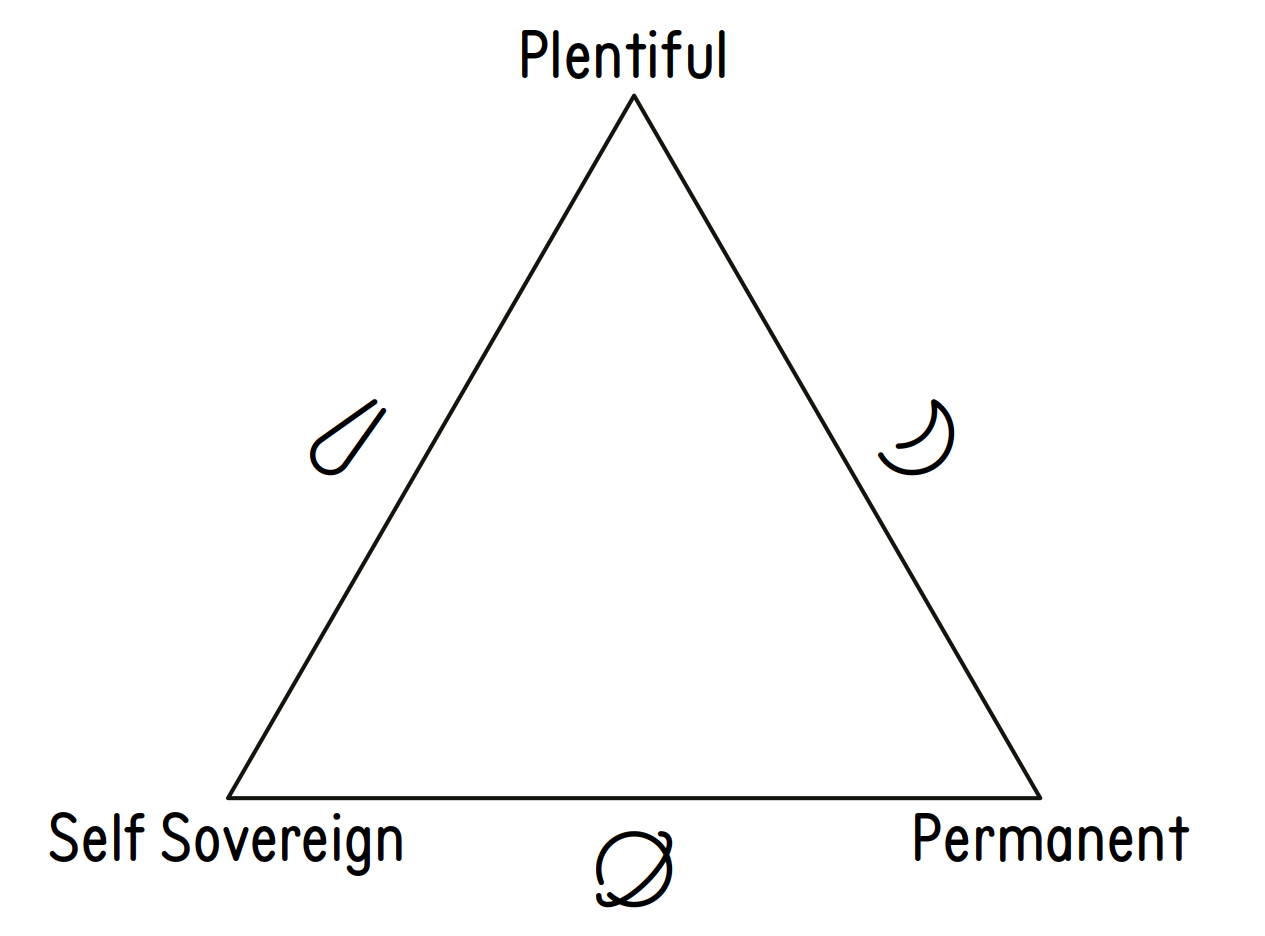
\includegraphics[width=\textwidth]{img/trilemma}
  \caption{Trilemma of properties for a sane network.}
  \label{fig:trilemma}
\end{figure}
  
To create a sane network, we require global consistency for all our
names (Figure \ref{fig:trilemma}). There are three other properties; pick any two:

\begin{itemize}
\item
  Comets are impermanent, self sovereign, and plentiful.
\item
  Planets are permanent, self sovereign, and not plentiful.
\item
  Moons are permanent, not self sovereign, and plentiful.
\end{itemize}

Fancifully, comets are wayward celestial bodies that are great for
testing and miscellaneous low-value things that won't last for long.
Planets are where you can build a home and shape it into anything you
want it to be. People can always find your planet; it's not going
anywhere. Moons are useful for special purposes, like storage, heavy
industry, and anything else you might want to do
off-planet.\footnote{To extend the metaphor, stars are a neighborhood to live in—they're
easier for other planets to see, so when they want to send you a
message they look for your star first. If they don't even know where
your star is, they can certainly find your star's galaxy, and that
will be enough to locate the star. Of course, if your star is not
providing satisfactory service, you can take your planet and move to
another star.} \tombstone{}

\selectlanguage{USenglish}
\printbibliography
\end{document}
